
\chapter{Background Theory}

\label{ch:background}

\section{Introduction}
Galaxy morphology has traditionally been classified based on the Hubble sequence, originating from the identification galaxy features from photographic plates. However, this classification is based on visual distinctions and fails to accurately represent early-type galaxies (E's and S0's) and it was argued by \cite{Cappellari2011} and \cite{Emsellem2011} that a more telling classification would be based on the spin parameter due to the intrinsic qualitative change in velocity structure exhibited by galaxies, with a threshold of separating slow ($\lambda<0.1$) and fast ($\geq0.1$) rotators. $\lambda_{R}$ is defined as\cite{sauron9}:
\begin{equation}
\lambda_{R} = \frac{\sum_{i=1}^{N_{p}} F_{i}R_{i}|V_{i}|}{\sum_{i=1}^{N_{p}}F_{i}R_{i}\sqrt{V_{i}^2+\sigma_{i}^2}}
\end{equation}
where $F_i$, $R_i$, $V_i$ and $σ_i$ are the flux, circular radius, velocity and velocity dispersion of the ith spatial bin, the sum running on the $N_p$ bins.
This is superior over a velocity dispersion classification, $V/\sigma$, which fails when confronted by galaxies with kinematically decouple cores (KDC), "whose angular momentum vector is misaligned with respect to that of the bulk of the galaxy" \cite{mo_bosch_white_2010}. Furthermore, $\lambda_{R}$ it was found 'we can quantify galaxy morphology via the kinematic properties of galaxies\cite{Cortese2016}[p14]', beyond early types. 
\begin{figure}[h]
	\caption{Galaxies from ATLAS$_{3D}$ colour coded by optical morphology. There appears a weak correlation for early types that grows more pronounced for early types.	
		 \cite{Cortese2016}[p12]}
	\centering
	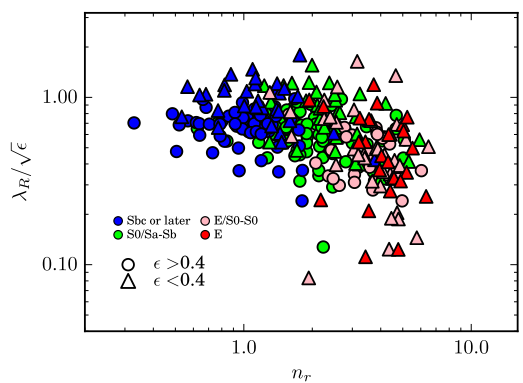
\includegraphics{morphology_sersic_cortese2016.png}
\end{figure}

(Although this paper suggests that the correlation breaks down for early types, others...DON'T INCLUDE THIS MAYBE...).  

\begin{figure}[h]
	\caption{Radial $\lambda_{R}$ profiles for the 48 E and S0 galaxies of the SAURON
	sample. Profiles of slow and fast rotators are coloured in red and blue, respectively.
	NGC numbers are indicated for all fast rotators and most slow
	rotators \cite[p.6]{Emsellem2011}}
	\centering
	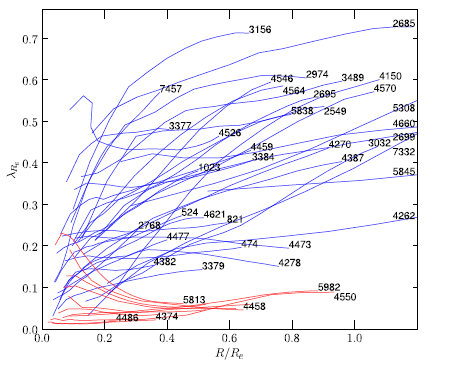
\includegraphics{fastslowemsellem2008.png}
\end{figure}

As can be seen in Fig 2.1, there appears a weak correlation for galaxies in the SAMI survey for early-type galaxies, but this becomes much stronger for late-types.
The spin parameter is costly to determine due to its reliance on integral field spectroscopy and has therefore only been found for a small number of galaxies: 260 from the ATLAS3D survey and 446 from SAMI. This compares with over 500 million galaxies with photometric data from the Sloan Digital Sky Survey (SDSS) alone \cite{SDSS}. Although other classifications do not rely on this parameter, it is still of value in relation to other properties. It is therefore of great value to find an alternative means of identifying the rotation.\
Although the motivation for this study is to extend identifying the spin parameter to all morphological classes, this paper will focus on the early-type galaxies taken from \cite{Emsellem2011}.
In \cite{Emsellem2008}, it was found that fast rotators tend to be relatively low luminosity with $M_{B}\lesssim-20.5$ and well aligned photometric and kinemetric axes, while slow rotators tend to be brighter and more massive galaxies, that exhibit either no rotation or KDC's.
In order to evaluate the rotation and its effect on observable parameters, it is necessary to consider the current understanding of galaxy morphology. The traditional means of classifying galaxies was based on the Hubble tuning fork that split galaxies into spiral and elliptical galaxies based on their visual morphological appearance.
#HUBBLE TUNING FORK IMAGE HERE
There are several reasons for this distinction. Spirals are generally younger galaxies with a net angular momentum and hence more likely to form discs on a plane coincident with this. FUCKIN REFERENCE
There have been a variety of methods of quantifying these classifications, but generally consists of identifying the different components of the galaxy, being the disk and the bulge, and their relative importance.  Several (MORE DETAIL HERE) properties of galaxies correlate with their classification, and the subject of this part of the paper will be to briefly describe how this is so (IMPROVE THE ABOVE PARAGRAPH).
\section{Measured Parameters}
The parameters used in modelling the data were:
\subsection{Variations of the Spin Parameter}
The ATLAS3D paper measured $\lambda$ to 1 effective radius, $R_{e}$ and to half the effective radius, $R_{e}/2$, where 
\begin{equation}
I(R_{e}=I_{0}/e)
\end{equation}
whereas the SAMI paper only measured this for $R_{e}$\cite[p.~3]{Cortese2016}. 
\subsection{S\'ersic Index of the Single Fit and Bulge Component, n and $n_{b}$}
The S\'ersic profile models the light intensity over the surface of the galaxy in terms of an exponential function as a function of the distance from the centre, R, and the S\'ersic index n:
\begin{equation}
I(R) = I_{e} exp\{-b_{n} [(R/R_{e})^{1/n}-1]\}
\end{equation}
The range of the S\'ersic index covers the full range from steep (i.e. concetrated n>>1) to shallow (n$\lesssim 1$) surface brightness profiles %\cite{lectures}.
Galaxies 
\begin{equation}
\lambda_{Re}=(0.31\pm0.01)
\end{equation}
\section{ATLAS$^{3D}$}
This survey combined 
According to \cite{Cappellari2011}
this survey focused on a 'volume-limited ($\num{1.16e05} Mpc^{3}$) sample of 260 early-type (elliptical E and lenticular S0) galaxies (ETGs)...The sample consists of nearby (D < 42 Mpc, $|\delta \num{-29}^{\circ}| < 35^{\circ}$, $|b| > 15^{\circ})$ morphologically selected ETG's extracted from a parent sample of 871 galaxies (8 per cent E, 22 per cent S0 and
70 per cent spirals) brighter than $M_{K} <\num{-21.5} $mag (stellar mass $M_{\star} \gtrsim \num{6e09} M_{\odot}$).' ETG's were defined as having de Vaucouleurs T type T > -3.5 and T $\leq -3.5$ for S0 and E galaxies respectively, which correlates with the Hubble classes, i.e. lenticulars and ellipticals.


